\section{Appendix: Code}
The following is a pdf of the Jupyter Notebook used for this assignment.
% Include all pages of the code PDF
% 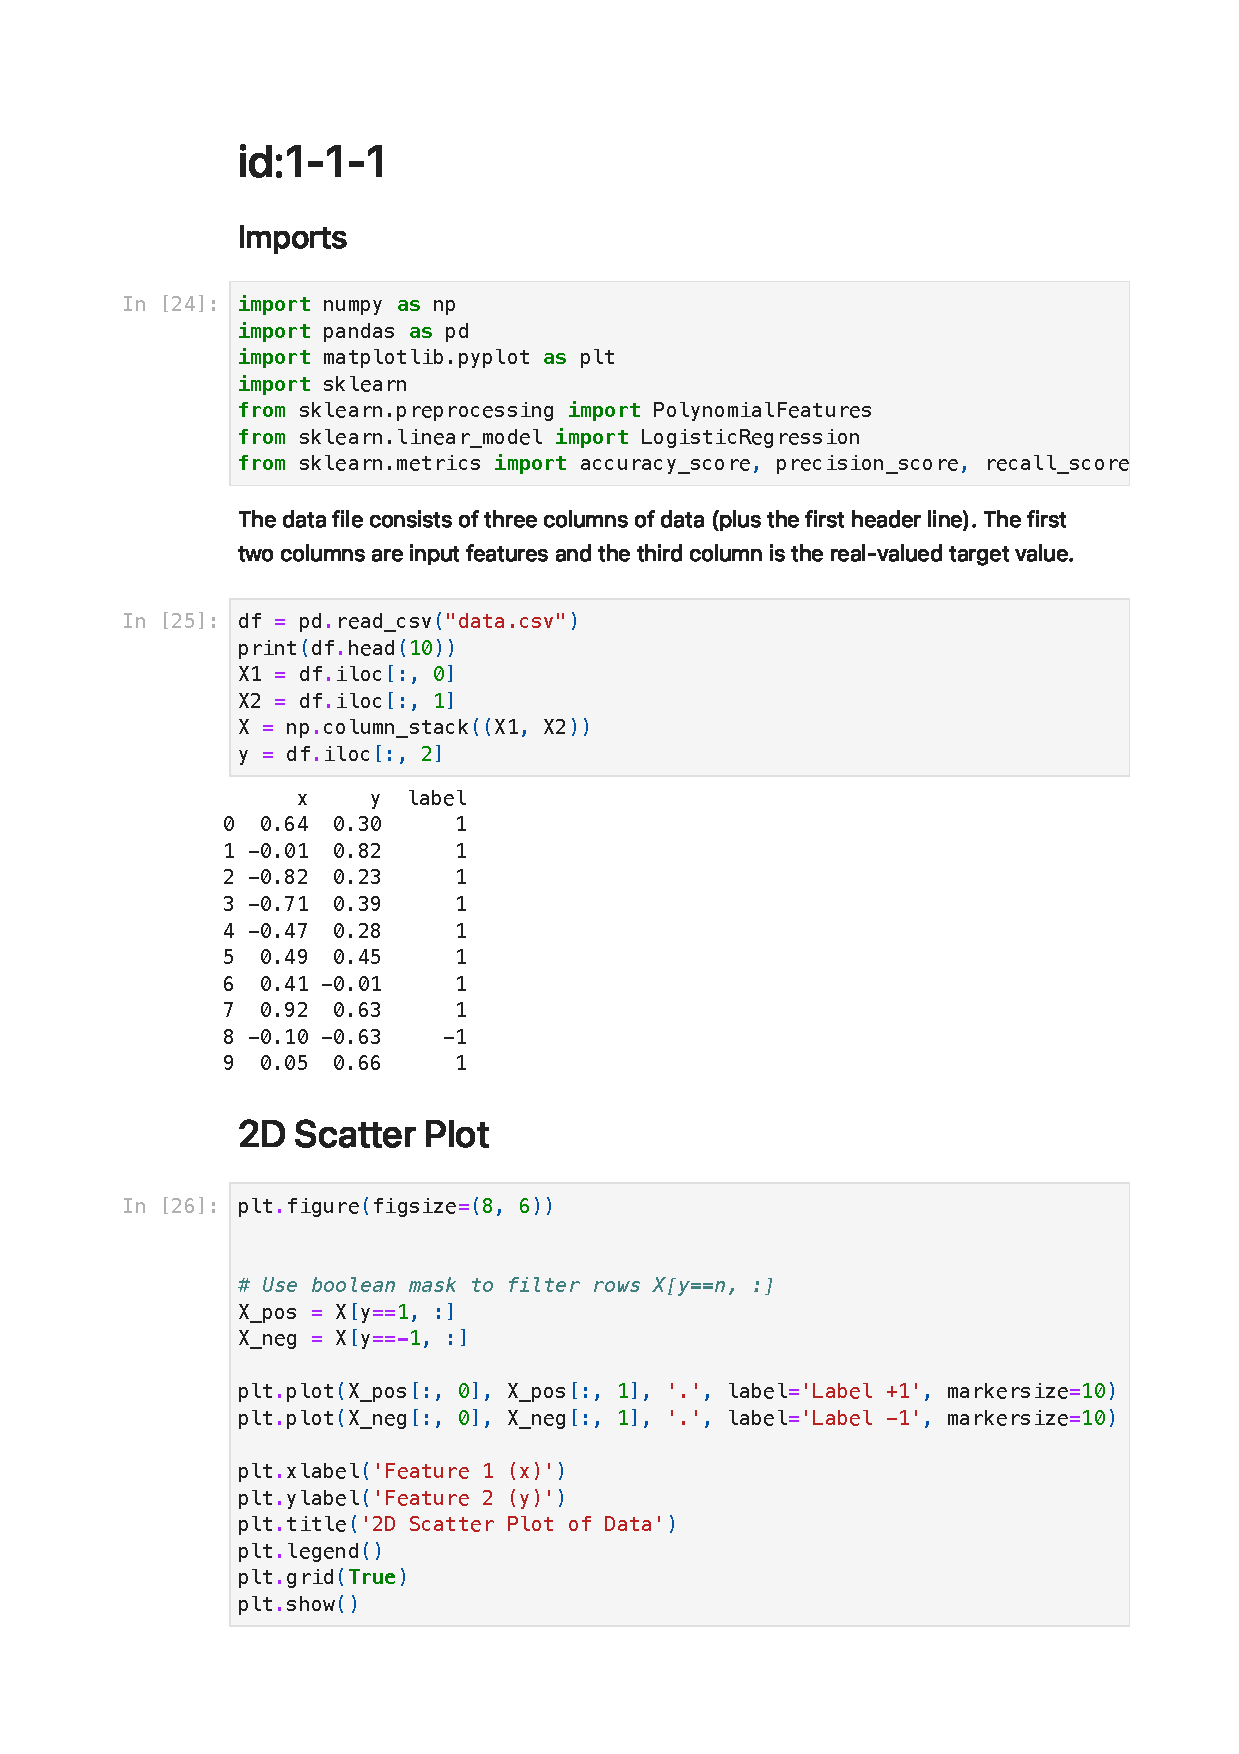
\includepdf[pages=-,pagecommand={}]{notebook/code.pdf}

\subsection{main.py}
\begin{verbatim}
    import torch
    import torch.nn as nn
    from torch.nn import functional as F
    import matplotlib.pyplot as plt
    import argparse
    import os
    import csv

    # hyperparameters
    batch_size = 64 # how many independent sequences will we process in parallel?
    block_size = 256 # what is the maximum context length for predictions?
    max_iters = 1000
    eval_interval = 10
    learning_rate = 3e-4
    eval_iters = 200
    n_embd = 128
    n_head = 4
    n_layer = 4
    dropout = 0.2

    if torch.cuda.is_available():
        device = 'cuda'
    elif torch.backends.mps.is_available():
        device = 'mps'
    else:
        device = 'cpu'
    # ------------

    parser = argparse.ArgumentParser(description='Train a model.')
    parser.add_argument('--plot', action='store_true', help='Save a plot of the loss.')
    parser.add_argument('--model', type=str, help='Path to a saved model to load for evaluation.')
    parser.add_argument('--FF_FACTOR', type=int, default=4, help='Feed forward factor.')
    # default bias to True; providing --bias will disable attention biases (store_false)
    parser.add_argument('--bias', action='store_false', help='Disable bias in attention layers.', default=True)
    parser.add_argument('--weight_tying', action='store_true', help='Enable weight tying.')
    # default skip connections to True; providing --skip will disable skip connections (store_false)
    parser.add_argument('--no_skip', action='store_false', help='Disable skip connections.', default=True)
    args = parser.parse_args()

    FF_FACTOR = args.FF_FACTOR
    bias_enabled = args.bias
    skip_enabled = args.no_skip

    print(f"Configuration: FF_FACTOR={FF_FACTOR}, weight_tying={args.weight_tying}, bias={bias_enabled}, skip={skip_enabled}")

    torch.manual_seed(1337)

    SHAKESPEAR = 'datasets/input_shakespeare.txt'
    CHILDSPEECH_TEST = 'datasets/input_childSpeech_testSet.txt'
    CHILDSPEECH_TRAIN = 'datasets/input_childSpeech_trainingSet.txt'

    # wget https://raw.githubusercontent.com/karpathy/char-rnn/master/data/tinyshakespeare/input.txt
    with open(CHILDSPEECH_TRAIN, 'r', encoding='utf-8') as f:
        text = f.read()

    # here are all the unique characters that occur in this text
    chars = sorted(list(set(text)))
    vocab_size = len(chars)
    # create a mapping from characters to integers
    stoi = { ch:i for i,ch in enumerate(chars) }
    itos = { i:ch for i,ch in enumerate(chars) }
    encode = lambda s: [stoi[c] for c in s] # encoder: take a string, output a list of integers
    decode = lambda l: ''.join([itos[i] for i in l]) # decoder: take a list of integers, output a string

    # Train and test splits
    data = torch.tensor(encode(text), dtype=torch.long)
    n = int(0.9*len(data)) # first 90% will be train, rest val
    train_data = data[:n]
    val_data = data[n:]

    # data loading
    def get_batch(split):
        # generate a small batch of data of inputs x and targets y
        data = train_data if split == 'train' else val_data
        ix = torch.randint(len(data) - block_size, (batch_size,))
        x = torch.stack([data[i:i+block_size] for i in ix])
        y = torch.stack([data[i+1:i+block_size+1] for i in ix])
        x, y = x.to(device), y.to(device)
        return x, y

    @torch.no_grad()
    def estimate_loss():
        out = {}
        model.eval()
        for split in ['train', 'val']:
            losses = torch.zeros(eval_iters)
            for k in range(eval_iters):
                X, Y = get_batch(split)
                logits, loss = model(X, Y)
                losses[k] = loss.item()
            out[split] = losses.mean()
        model.train()
        return out

    class Head(nn.Module):
        """ one head of self-attention """

        def __init__(self, head_size):
            super().__init__()
            self.key = nn.Linear(n_embd, head_size, bias=bias_enabled)
            self.query = nn.Linear(n_embd, head_size, bias=bias_enabled)
            self.value = nn.Linear(n_embd, head_size, bias=bias_enabled)
            self.register_buffer('tril', torch.tril(torch.ones(block_size, block_size)))

            self.dropout = nn.Dropout(dropout)

        def forward(self, x):
            # input of size (batch, time-step, channels)
            # output of size (batch, time-step, head size)
            B,T,C = x.shape
            k = self.key(x)   # (B,T,hs)
            q = self.query(x) # (B,T,hs)
            # compute attention scores ("affinities")
            wei = q @ k.transpose(-2,-1) * k.shape[-1]**-0.5 # (B, T, hs) @ (B, hs, T) -> (B, T, T)
            wei = wei.masked_fill(self.tril[:T, :T] == 0, float('-inf')) # (B, T, T)
            wei = F.softmax(wei, dim=-1) # (B, T, T)
            wei = self.dropout(wei)
            # perform the weighted aggregation of the values
            v = self.value(x) # (B,T,hs)
            out = wei @ v # (B, T, T) @ (B, T, hs) -> (B, T, hs)
            return out

    class MultiHeadAttention(nn.Module):
        """ multiple heads of self-attention in parallel """

        def __init__(self, num_heads, head_size):
            super().__init__()
            self.heads = nn.ModuleList([Head(head_size) for _ in range(num_heads)])
            self.proj = nn.Linear(head_size * num_heads, n_embd)
            self.dropout = nn.Dropout(dropout)

        def forward(self, x):
            out = torch.cat([h(x) for h in self.heads], dim=-1)
            out = self.dropout(self.proj(out))
            return out

    class FeedFoward(nn.Module):
        """ a simple linear layer followed by a non-linearity """

        def __init__(self, n_embd):
            super().__init__()
            
            # Feed Forward network
            self.net = nn.Sequential(
                nn.Linear(n_embd, FF_FACTOR * n_embd),
                nn.ReLU(),
                nn.Linear(FF_FACTOR * n_embd, n_embd),
                nn.Dropout(dropout),
            )

        def forward(self, x):
            return self.net(x)

    class Block(nn.Module):
        """ Transformer block: communication followed by computation """

        def __init__(self, n_embd, n_head):
            # n_embd: embedding dimension, n_head: the number of heads we'd like
            super().__init__()
            head_size = n_embd // n_head
            self.sa = MultiHeadAttention(n_head, head_size)
            self.ffwd = FeedFoward(n_embd)
            self.ln1 = nn.LayerNorm(n_embd)
            self.ln2 = nn.LayerNorm(n_embd)

        def forward(self, x):
            if skip_enabled:
                x = x + self.sa(self.ln1(x))
                x = x + self.ffwd(self.ln2(x))
            else:
                # run the sublayers without residual additions
                x = self.sa(self.ln1(x))
                x = self.ffwd(self.ln2(x))
            return x

    class GPTLanguageModel(nn.Module):

        def __init__(self):
            super().__init__()
            # each token directly reads off the logits for the next token from a lookup table
            self.token_embedding_table = nn.Embedding(vocab_size, n_embd)
            self.position_embedding_table = nn.Embedding(block_size, n_embd)
            self.blocks = nn.Sequential(*[Block(n_embd, n_head=n_head) for _ in range(n_layer)])
            self.ln_f = nn.LayerNorm(n_embd) # final layer norm
            self.lm_head = nn.Linear(n_embd, vocab_size)

            if args.weight_tying:
                self.lm_head.weight = self.token_embedding_table.weight

            # better init, not covered in the original GPT video, but important, will cover in followup video
            self.apply(self._init_weights)

        def _init_weights(self, module):
            if isinstance(module, nn.Linear):
                torch.nn.init.normal_(module.weight, mean=0.0, std=0.02)
                if module.bias is not None:
                    torch.nn.init.zeros_(module.bias)
            elif isinstance(module, nn.Embedding):
                torch.nn.init.normal_(module.weight, mean=0.0, std=0.02)

        def forward(self, idx, targets=None):
            B, T = idx.shape

            # idx and targets are both (B,T) tensor of integers
            tok_emb = self.token_embedding_table(idx) # (B,T,C)
            pos_emb = self.position_embedding_table(torch.arange(T, device=device)) # (T,C)
            x = tok_emb + pos_emb # (B,T,C)
            x = self.blocks(x) # (B,T,C)
            x = self.ln_f(x) # (B,T,C)
            logits = self.lm_head(x) # (B,T,vocab_size)

            if targets is None:
                loss = None
            else:
                B, T, C = logits.shape
                logits = logits.view(B*T, C)
                targets = targets.view(B*T)
                loss = F.cross_entropy(logits, targets)

            return logits, loss

        def generate(self, idx, max_new_tokens):
            # idx is (B, T) array of indices in the current context
            for _ in range(max_new_tokens):
                # crop idx to the last block_size tokens
                idx_cond = idx[:, -block_size:]
                # get the predictions
                logits, loss = self(idx_cond)
                # focus only on the last time step
                logits = logits[:, -1, :] # becomes (B, C)
                # apply softmax to get probabilities
                probs = F.softmax(logits, dim=-1) # (B, C)
                # sample from the distribution
                idx_next = torch.multinomial(probs, num_samples=1) # (B, 1)
                # append sampled index to the running sequence
                idx = torch.cat((idx, idx_next), dim=1) # (B, T+1)
            return idx

    model = GPTLanguageModel()
    m = model.to(device)

    if args.model:
        print(f"Loading model from {args.model}")
        try:
            model.load_state_dict(torch.load(args.model, map_location=device))
        except RuntimeError as e:
            print(f"Strict loading failed (likely config mismatch): {e}")
            print("Attempting to load with strict=False (ignoring missing keys, e.g. biases)...")
            model.load_state_dict(torch.load(args.model, map_location=device), strict=False)

    # print the number of parameters in the model
    print(sum(p.numel() for p in m.parameters())/1e6, 'M parameters')

    if not args.model:
        # create a PyTorch optimizer
        optimizer = torch.optim.AdamW(model.parameters(), lr=learning_rate)

        train_losses = []
        val_losses = []
        steps = []

        for iter in range(max_iters):

            # every once in a while evaluate the loss on train and val sets
            if iter % eval_interval == 0 or iter == max_iters - 1:
                losses = estimate_loss()
                print(f"step {iter}: train loss {losses['train']:.4f}, val loss {losses['val']:.4f}")
                steps.append(iter)
                train_losses.append(losses['train'])
                val_losses.append(losses['val'])

            # sample a batch of data
            xb, yb = get_batch('train')

            # evaluate the loss
            logits, loss = model(xb, yb)
            optimizer.zero_grad(set_to_none=True)
            loss.backward()
            optimizer.step()

        # Save model and hyperparameters
        os.makedirs('models', exist_ok=True)
        dataset_name = os.path.splitext(os.path.basename(CHILDSPEECH_TRAIN))[0]
        model_path = os.path.join('models', f'model_{dataset_name}.pt')
        torch.save(model.state_dict(), model_path)
        print(f"Model saved to {model_path}")

        if args.plot:
            # Create and save the final plot
            fig, ax = plt.subplots()
            ax.plot(steps, train_losses, label='train loss')
            ax.plot(steps, val_losses, label='val loss')
            ax.legend()
            ax.set_xlabel('Steps')
            ax.set_ylabel('Loss')
            ax.set_title('Training and Validation Loss')
            plot_path = os.path.join('models', f'loss_curve_{dataset_name}.png')
            plt.savefig(plot_path)
            plt.close()
            print(f"Loss curve saved to {plot_path}")

            csv_path = os.path.join('models', f'loss_data_{dataset_name}.csv')
            with open(csv_path, 'w', newline='') as f:
                writer = csv.writer(f)
                writer.writerow(['step', 'train_loss', 'val_loss'])
                for s, t, v in zip(steps, train_losses, val_losses):
                    writer.writerow([s, t.item(), v.item()])
            print(f"Loss data saved to {csv_path}")

        params_path = os.path.join('models', f'model_{dataset_name}_params.txt')
        with open(params_path, 'w') as f:
            f.write(f"batch_size: {batch_size}\n")
            f.write(f"block_size: {block_size}\n")
            f.write(f"max_iters: {max_iters}\n")
            f.write(f"learning_rate: {learning_rate}\n")
            f.write(f"n_embd: {n_embd}\n")
            f.write(f"n_head: {n_head}\n")
            f.write(f"n_layer: {n_layer}\n")
            f.write(f"dropout: {dropout}\n")
            f.write(f"FF_FACTOR: {FF_FACTOR}\n")
            f.write(f"weight_tying: {args.weight_tying}\n")
            f.write(f"bias: {bias_enabled}\n")
            f.write(f"skip: {skip_enabled}\n")
            f.write(f"vocab_size: {vocab_size}\n")
            f.write(f"device: {device}\n")

    # generate from the model
    context = torch.zeros((1, 1), dtype=torch.long, device=device)
    print(decode(m.generate(context, max_new_tokens=500)[0].tolist()))
    #open('more.txt', 'w').write(decode(m.generate(context, max_new_tokens=10000)[0].tolist()))
\end{verbatim}


\subsection{Evaluation.py}

\begin{verbatim}
    import os
    import math
    import argparse
    import torch
    import torch.nn as nn
    from torch.nn import functional as F

    def read_params(params_path):
        params = {}
        with open(params_path, 'r') as f:
            for line in f:
                if ':' in line:
                    k, v = line.strip().split(':', 1)
                    params[k.strip()] = v.strip()
        return params

    # Minimal model code (kept in-sync with your training script).
    class Head(nn.Module):
        def __init__(self, n_embd, head_size, block_size, dropout, bias):
            super().__init__()
            self.key = nn.Linear(n_embd, head_size, bias=bias)
            self.query = nn.Linear(n_embd, head_size, bias=bias)
            self.value = nn.Linear(n_embd, head_size, bias=bias)
            self.register_buffer('tril', torch.tril(torch.ones(block_size, block_size)))
            self.dropout = nn.Dropout(dropout)
        def forward(self, x):
            B,T,C = x.shape
            k = self.key(x)
            q = self.query(x)
            wei = q @ k.transpose(-2,-1) * k.shape[-1]**-0.5
            wei = wei.masked_fill(self.tril[:T, :T] == 0, float('-inf'))
            wei = F.softmax(wei, dim=-1)
            wei = self.dropout(wei)
            v = self.value(x)
            out = wei @ v
            return out

    class MultiHeadAttention(nn.Module):
        def __init__(self, n_embd, num_heads, head_size, block_size, dropout, bias):
            super().__init__()
            self.heads = nn.ModuleList([Head(n_embd, head_size, block_size, dropout, bias) for _ in range(num_heads)])
            self.proj = nn.Linear(head_size * num_heads, n_embd)
            self.dropout = nn.Dropout(dropout)
        def forward(self, x):
            out = torch.cat([h(x) for h in self.heads], dim=-1)
            out = self.dropout(self.proj(out))
            return out

    class FeedFoward(nn.Module):
        def __init__(self, n_embd, ff_factor, dropout):
            super().__init__()
            self.net = nn.Sequential(
                nn.Linear(n_embd, ff_factor * n_embd),
                nn.ReLU(),
                nn.Linear(ff_factor * n_embd, n_embd),
                nn.Dropout(dropout),
            )
        def forward(self, x):
            return self.net(x)

    class Block(nn.Module):
        def __init__(self, n_embd, n_head, ff_factor, block_size, dropout, bias, skip_enabled):
            super().__init__()
            head_size = n_embd // n_head
            self.sa = MultiHeadAttention(n_embd, n_head, head_size, block_size, dropout, bias)
            self.ffwd = FeedFoward(n_embd, ff_factor, dropout)
            self.ln1 = nn.LayerNorm(n_embd)
            self.ln2 = nn.LayerNorm(n_embd)
            self.skip_enabled = skip_enabled
        def forward(self, x):
            if self.skip_enabled:
                x = x + self.sa(self.ln1(x))
                x = x + self.ffwd(self.ln2(x))
            else:
                x = self.sa(self.ln1(x))
                x = self.ffwd(self.ln2(x))
            return x

    class GPTLanguageModel(nn.Module):
        def __init__(self, vocab_size, block_size, n_embd, n_head, n_layer, ff_factor, dropout, bias, weight_tying, skip_enabled):
            super().__init__()
            self.token_embedding_table = nn.Embedding(vocab_size, n_embd)
            self.position_embedding_table = nn.Embedding(block_size, n_embd)
            self.blocks = nn.Sequential(*[Block(n_embd, n_head, ff_factor, block_size, dropout, bias, skip_enabled) for _ in range(n_layer)])
            self.ln_f = nn.LayerNorm(n_embd)
            self.lm_head = nn.Linear(n_embd, vocab_size)
            if weight_tying:
                # tie weights
                self.lm_head.weight = self.token_embedding_table.weight
            # init (same scheme as training script)
            self.apply(self._init_weights)
        def _init_weights(self, module):
            if isinstance(module, nn.Linear):
                torch.nn.init.normal_(module.weight, mean=0.0, std=0.02)
                if module.bias is not None:
                    torch.nn.init.zeros_(module.bias)
            elif isinstance(module, nn.Embedding):
                torch.nn.init.normal_(module.weight, mean=0.0, std=0.02)

        def generate(self, idx, max_new_tokens):
            # idx is (B, T) array of indices in the current context
            for _ in range(max_new_tokens):
                # crop idx to the last block_size tokens
                idx_cond = idx[:, -self.position_embedding_table.num_embeddings:]
                # get the predictions
                logits, _ = self(idx_cond)
                # focus only on the last time step
                logits = logits[:, -1, :] # becomes (B, C)
                # apply softmax to get probabilities
                probs = F.softmax(logits, dim=-1) # (B, C)
                # sample from the distribution
                idx_next = torch.multinomial(probs, num_samples=1) # (B, 1)
                # append sampled index to the running sequence
                idx = torch.cat((idx, idx_next), dim=1) # (B, T+1)
            return idx

        def forward(self, idx, targets=None):
            B,T = idx.shape
            tok_emb = self.token_embedding_table(idx)
            pos_emb = self.position_embedding_table(torch.arange(T, device=idx.device))
            x = tok_emb + pos_emb
            x = self.blocks(x)
            x = self.ln_f(x)
            logits = self.lm_head(x)
            if targets is None:
                return logits, None
            B,T,C = logits.shape
            logits = logits.view(B*T, C)
            targets = targets.view(B*T)
            loss = F.cross_entropy(logits, targets)
            return logits.view(B,T,C), loss

    # helpers for tokenization (use same training file to build vocab)
    def build_vocab_from_training(training_path):
        with open(training_path, 'r', encoding='utf-8') as f:
            text = f.read()
        chars = sorted(list(set(text)))
        stoi = { ch:i for i,ch in enumerate(chars) }
        itos = { i:ch for i,ch in enumerate(chars) }
        return stoi, itos

    def text_to_tensor(path, stoi, device, allow_unk=False):
        with open(path, 'r', encoding='utf-8') as f:
            text = f.read()
        unique_chars = sorted(set(text))
        missing = [c for c in unique_chars if c not in stoi]
        if missing and not allow_unk:
            # give a clear, actionable error instead of KeyError
            missing_display = ', '.join(sorted(missing))
            raise RuntimeError(
                f"Found characters in {os.path.basename(path)} that are not in the model vocabulary: {missing_display}\n"
                "Suggestions:\n"
                " - Re-run evaluation with --training_text pointing to the exact training text used to build the model's vocab\n"
                " - Build a combined training vocab that includes both the training and test texts\n"
                " - If you understand the consequences, re-run with --allow_unk to map unknown chars to a fallback index (0) and proceed\n"
            )
        # map text to indices; if allow_unk map unknowns to index 0
        if allow_unk and missing:
            # SKIP unknown characters instead of mapping to 0
            mapped = [stoi[c] for c in text if c in stoi]
            print(f"Warning: {len(missing)} unique characters not in vocab; skipping {len(text) - len(mapped)} occurrences for evaluation.")
        else:
            mapped = [stoi[c] for c in text]
        data = torch.tensor(mapped, dtype=torch.long)
        return data.to(device)

    def sequential_batches(data, block_size, batch_size):
        # produce non-overlapping sequential batches until exhaustion
        n = len(data)
        # compute number of full blocks
        max_start = n - block_size - 1
        if max_start < 0:
            return
        starts = list(range(0, max_start+1, block_size))
        for i in range(0, len(starts), batch_size):
            batch_starts = starts[i:i+batch_size]
            xb = torch.stack([data[s:s+block_size] for s in batch_starts])
            yb = torch.stack([data[s+1:s+block_size+1] for s in batch_starts])
            yield xb, yb

    def evaluate_model_on_file(model, data_tensor, block_size, batch_size, device):
        model.eval()
        total_loss = 0.0
        total_tokens = 0
        with torch.no_grad():
            for xb, yb in sequential_batches(data_tensor, block_size, batch_size):
                xb = xb.to(device)
                yb = yb.to(device)
                _, loss = model(xb, yb)
                if loss is None:
                    continue
                B,T = xb.shape
                total_loss += loss.item() * (B * T)
                total_tokens += (B * T)
        if total_tokens == 0:
            return float('nan')
        return total_loss / total_tokens

    def main():
        parser = argparse.ArgumentParser(description='Evaluate saved model on test sets.')
        parser.add_argument('--model', type=str, required=True, help='Path to saved .pt model to evaluate')
        parser.add_argument('--batch_size', type=int, default=64, help='Batch size for evaluation')
        parser.add_argument('--training_text', type=str, default='datasets/input_childSpeech_trainingSet.txt', help='Training text used to build vocab')
        parser.add_argument('--test_shakespeare', type=str, default='datasets/input_shakespeare.txt')
        parser.add_argument('--test_child', type=str, default='datasets/input_childSpeech_testSet.txt')
        parser.add_argument('--allow_unk', action='store_true', help='Map characters not in vocab to index 0 instead of failing')
        args = parser.parse_args()

        model_path = args.model
        if not os.path.isfile(model_path):
            print('Model file not found:', model_path)
            return

        params_path = model_path.replace('.pt', '_params.txt')
        if not os.path.isfile(params_path):
            print('Params file not found alongside model. Expected:', params_path)
            return

        params = read_params(params_path)
        # get required params with fallbacks
        block_size = params.get('block_size', 256)
        n_embd = params.get('n_embd', 128)
        n_head = params.get('n_head', 4)
        n_layer = params.get('n_layer', 4)
        ff_factor = params.get('FF_FACTOR', 4)
        dropout = float(params.get('dropout', 0.2)) if 'dropout' in params else 0.2
        bias = params.get('bias', True)
        weight_tying = params.get('weight_tying', False)
        skip_enabled = params.get('skip', True)
        vocab_size = params.get('vocab_size', None)
        device_name = params.get('device', None)

        # pick device
        if device_name == 'cuda' and torch.cuda.is_available():
            device = torch.device('cuda')
        elif device_name == 'mps' and torch.backends.mps.is_available():
            device = torch.device('mps')
        else:
            device = torch.device('cpu')

        # Build vocab from training text to ensure consistent stoi/itos
        stoi, itos = build_vocab_from_training(args.training_text)
        if vocab_size is None:
            vocab_size = len(stoi)
        else:
            if int(vocab_size) != len(stoi):
                print('Warning: params vocab_size does not match training vocab. Using training vocab.')
                vocab_size = len(stoi)

        # instantiate model with matching hyperparams
        model = GPTLanguageModel(vocab_size=vocab_size, block_size=block_size, n_embd=n_embd,
                                n_head=n_head, n_layer=n_layer, ff_factor=ff_factor,
                                dropout=dropout, bias=bias, weight_tying=weight_tying, skip_enabled=skip_enabled)
        model = model.to(device)

        # load checkpoint
        sd = torch.load(model_path, map_location=device)
        try:
            model.load_state_dict(sd)
            print('Loaded checkpoint (strict=True).')
        except RuntimeError as e:
            print('Strict load failed:', e)
            try:
                model.load_state_dict(sd, strict=False)
                print('Loaded checkpoint with strict=False (some keys missing or unexpected).')
            except Exception as e2:
                print('Failed to load checkpoint:', e2)
                return

        # prepare test tensors
        test_shakespeare = text_to_tensor(args.test_shakespeare, stoi, device, allow_unk=args.allow_unk)
        test_child = text_to_tensor(args.test_child, stoi, device, allow_unk=args.allow_unk)

        print('Evaluating model on test sets...')
        bs = args.batch_size
        loss_child = evaluate_model_on_file(model, test_child, block_size, bs, device)

        # dummy uniform model loss (nats per token)
        dummy_loss = math.log(vocab_size)

        print('Results (cross-entropy nats per token):')
        print(f'  Model ({os.path.basename(model_path)}): Shakespeare loss = {loss_shakespeare:.6f}, ChildSpeech loss = {loss_child:.6f}')
        print(f'  Dummy uniform loss = {dummy_loss:.6f}')
        print(f'  Difference model - dummy : Shakespeare = {loss_shakespeare - dummy_loss:.6f}, ChildSpeech = {loss_child - dummy_loss:.6f}')

        print('\nGenerated Output:')
        decode = lambda l: ''.join([itos[i] for i in l])
        context = torch.zeros((1, 1), dtype=torch.long, device=device)
        print(decode(model.generate(context, max_new_tokens=500)[0].tolist()))

    if __name__ == '__main__':
        main()
\end{verbatim}

